\chapter{Análise do Problema}
\section{Descrição do Problema}
O principal problema a ser resolvido pela turma B é garantir que as medições de temperatura e pressão durante a execução de testes com combustão sejam confiáveis.

Em um grupo com alunos de Engenharias distintas, é necessário usar uma ferramenta para melhorar a compreensão do projeto. Para a documentação do problema foi escolhido o fishbone (diagrama de Ishikawa). Segue abaixo o resultado:

\begin{figure}[!htb]                                                               
   \centering                                                                      
   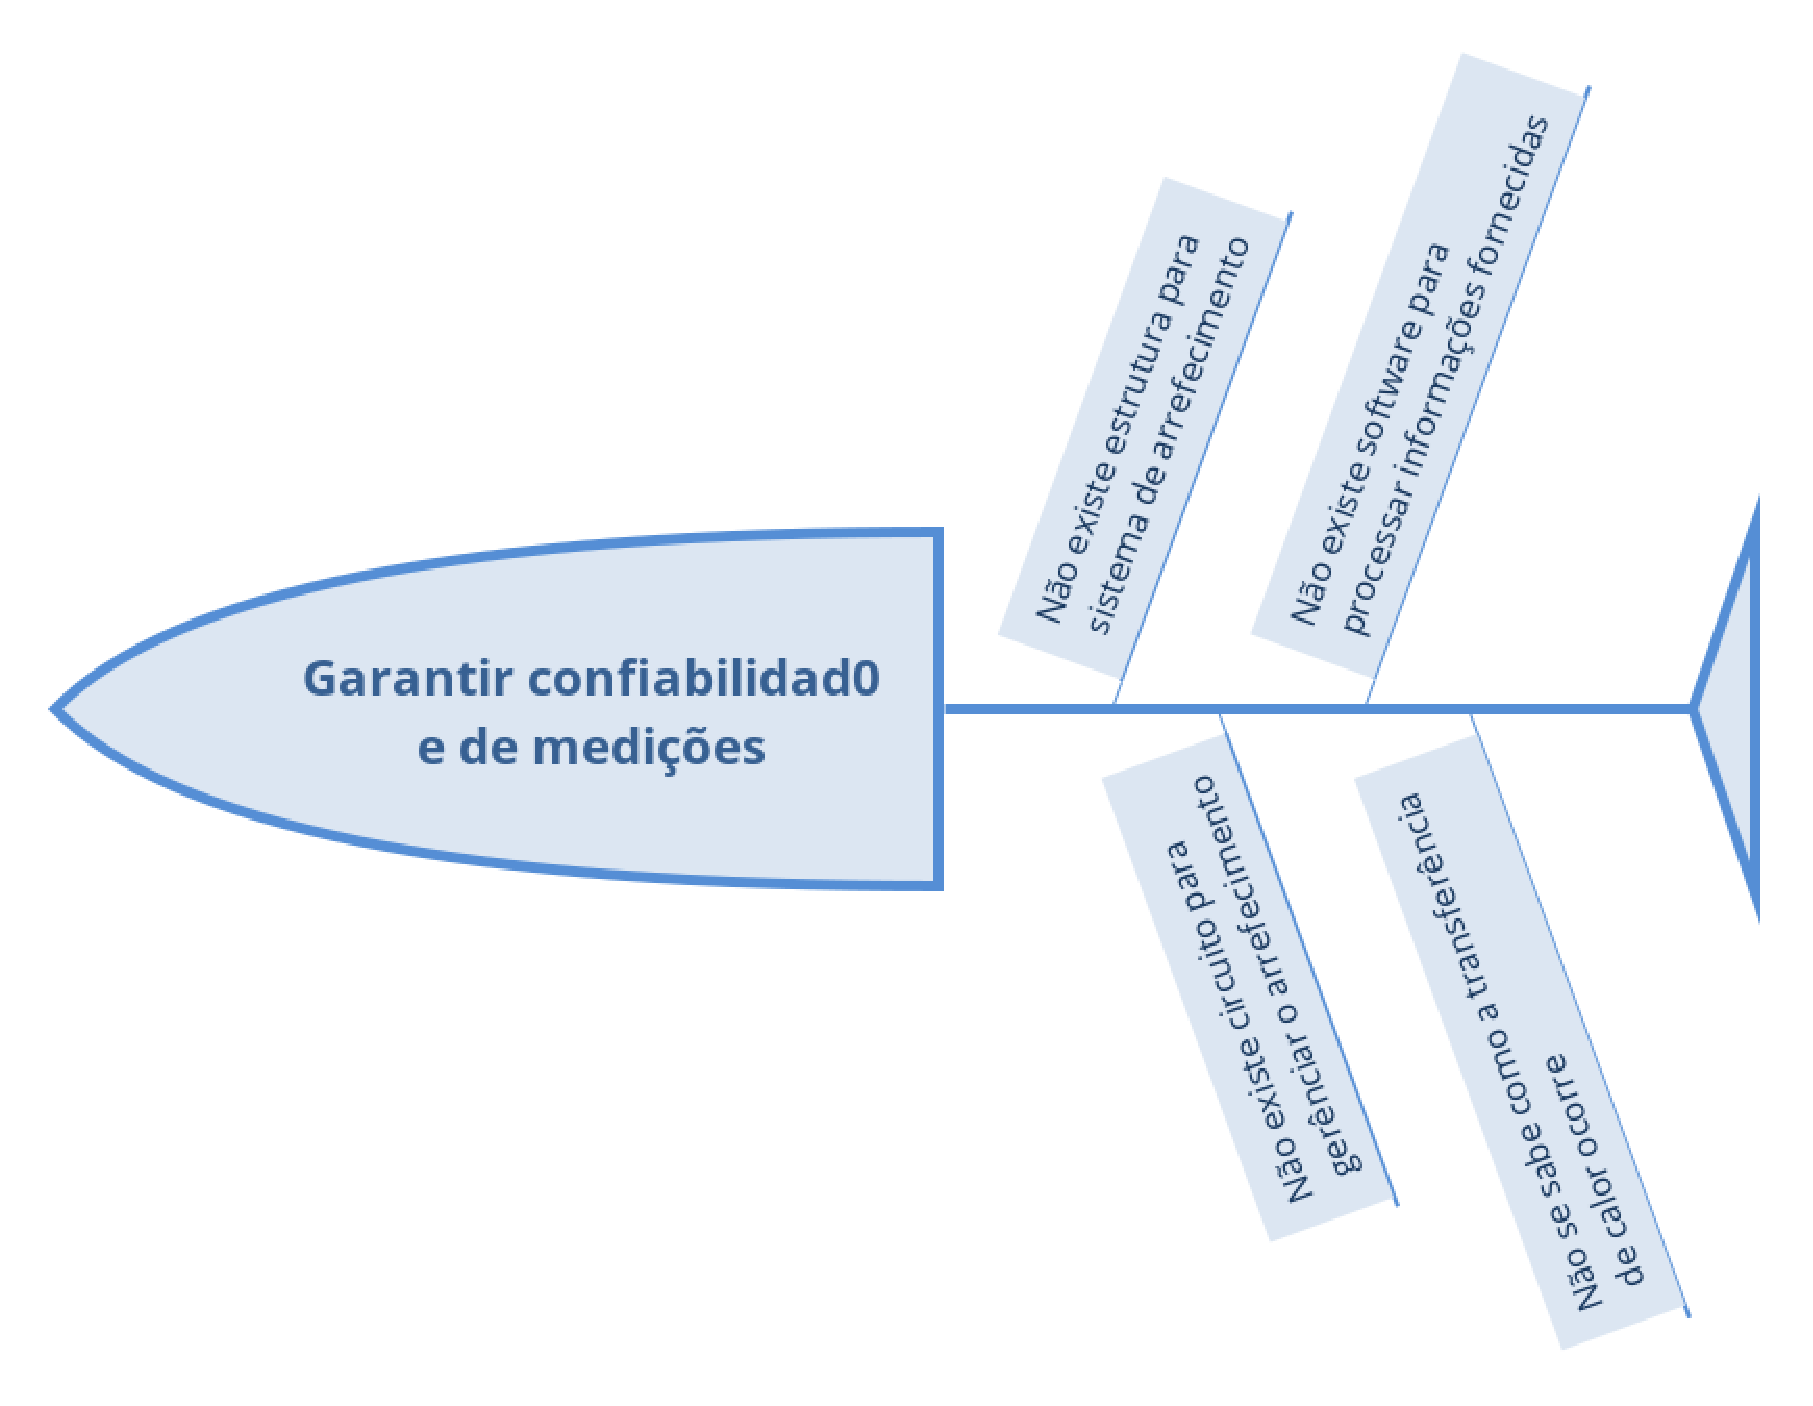
\includegraphics[width=15cm, keepaspectratio=true]{figuras/fishbone_pi1.eps}
   \caption{Visão de dependência entre as tarefas e prazos}                        
\end{figure}
